\documentclass[]{article}
\usepackage[spanish]{babel}  % Paquete para el idioma español
\usepackage{fancyhdr}  % Paquete para personalizar encabezados y pies de página
\usepackage{hyperref}
\usepackage{graphicx}
\usepackage{float}
\usepackage[backend=biber]{biblatex}

%opening
\title{Accesibilidad y normativa. Análisis de aplicaciones.}
\author{Imanol Benito Quintero Bermúdez}

\pagestyle{fancy}  % Activar el uso de fancyhdr
\fancyhf{}  % Limpiar encabezado y pie de página
\fancyhead[L]{Imanol Benito Quintero Bermúdez}  % Encabezado izquierdo
\fancyhead[R]{EII-ULPGC, PAMN 2024/2025}  % Encabezado derecho
\fancyfoot[C]{\thepage}  % Colocar número de página centrado en el pie
\setcounter{page}{2}  % Comenzar la numeración de página desde 2

\addto\captionsspanish{\renewcommand{\contentsname}{Índice}}  % Cambiar 'Contents' a 'Índice'

\begin{document}

\maketitle

\begin{abstract}
	La accesibilidad web es un principio fundamental que busca asegurar que cualquier persona, independientemente de sus capacidades físicas o cognitivas, pueda interactuar de manera efectiva con sitios y aplicaciones en línea. 
	
	En este proyecto, se analiza la accesibilidad del sitio web oficial del \textit{Congreso de los Diputados} (\href{https://www.congreso.es/es/home}{congreso.es}) y de la aplicación móvil de estadísticas deportivas \textit{\href{https://play.google.com/store/apps/details?id=com.sofascore.results&pcampaignid=web_share}{Sofascore}} con el objetivo de evaluar su conformidad con las Pautas de Accesibilidad para el Contenido Web (WCAG) y proponer mejoras que puedan facilitar su acceso a todos los usuarios.
	
	\begin{figure}[h]
		\centering
		
\includegraphics[width=\textwidth]{Capturas/5.png}
		\caption{Entrada principal del Palacio de las Cortes, en Madrid, presidida por dos grandes leones de bronce, Daoíz y Velarde}
		\label{fig:etiqueta}
	\end{figure}
\end{abstract}

\newpage  % Este comando hace que la introducción comience en una nueva página

\tableofcontents  % Genera la tabla de contenidos

\newpage

\section{Introducción}
En nuestra vida cotidiana, ya sea caminando por la calle, comprando en un comercio o asistiendo a clases, es común interactuar y compartir espacios con personas que tienen alguna discapacidad física, sensorial o intelectual. Según datos de la \textit{Organización Mundial de la Salud} (OMS), alrededor de 1.300 millones de personas, lo que representa el 16\% de la población mundial, vive con una discapacidad significativa. Este número destaca la importancia de crear entornos que sean accesibles para todos, permitiendo que todas las personas participen plenamente en la sociedad.

De hecho, cada vez es más habitual ver cómo los espacios físicos en grandes ciudades, como edificios públicos, viviendas y comercios, adaptan sus estructuras para cumplir con las necesidades de accesibilidad. Sin embargo, en una sociedad digitalizada como la actual, donde en España el 99,2\% de las personas de entre 16 y 74 años utilizan tecnologías de la información y la comunicación (TIC), la accesibilidad digital aún es un reto para muchas instituciones y empresas. Muchos sitios web y aplicaciones no han adaptado sus interfaces para incluir a personas con discapacidades, creando barreras en un ámbito tan fundamental como es el acceso a la información y los servicios en línea.

La accesibilidad web busca eliminar estos obstáculos, asegurando que cualquier persona, independientemente de sus capacidades físicas o cognitivas, pueda interactuar de manera eficiente con los sitios y aplicaciones en línea. Esto implica que las personas con discapacidades visuales, auditivas, motoras o cognitivas puedan acceder sin problemas a la información y realizar acciones en la web. A medida que el mundo digital crece, es imprescindible que los sitios cumplan con las \textit{Pautas de Accesibilidad para el Contenido Web} (WCAG), que establecen cuatro principios fundamentales: los sitios deben ser perceptibles, operables, comprensibles y robustos.

La accesibilidad web no solo mejora la experiencia de las personas con discapacidades, sino que también favorece a todos los usuarios, ya que un diseño más claro y estructurado facilita la navegación y el acceso a la información. Además, implementar accesibilidad no solo es un acto de justicia e inclusión social, sino que también amplía el alcance de los sitios web, permitiendo llegar a una audiencia más diversa.

Este trabajo tiene como objetivo evaluar la accesibilidad del sitio web del \textit{Congreso de los Diputados} (\href{https://www.congreso.es/es/home}{congreso.es}) y la aplicación móvil de resultados deportivos \textit{\href{https://play.google.com/store/apps/details?id=com.sofascore.results&pcampaignid=web_share}{Sofascore}} mediante diversas herramientas de análisis. Estas herramientas permitirán identificar y proponer soluciones a los problemas de accesibilidad relacionados con el diseño visual, la navegación y la compatibilidad con tecnologías de asistencia. La finalidad es evaluar el grado de conformidad del sitio con las pautas WCAG y sugerir mejoras que garanticen un acceso inclusivo para todos los usuarios.

\newpage

\section{WCAG: qué es y su utilidad}
\subsection*{¿Qué es WCAG?}

Los documentos denominados Pautas de Accesibilidad al Contenido en la Web (\textit{Web Content Accessibility Guidelines}, WCAG) explican cómo hacer que el contenido Web sea accesible para personas con discapacidad. El término \textit{contenido web} normalmente hace referencia a la información contenida en una página web o en una aplicación web, incluyendo texto, imágenes, formularios, sonido, y demás.

Las WCAG son parte de una serie de pautas de accesibilidad, que incluyen las Pautas de Accesibilidad para Herramientas de Autor (\textit{Authoring Tool Accessibility Guidelines}, ATAG) y las Pautas de Accesibilidad para Agentes de Usuario (\textit{User Agent Accessibility Guidelines}, UAAG). El documento \textit{Essential Components of Web Accessibility} explica la relación entre las diferentes pautas.

\subsection*{¿Quién crea las WCAG?}

Los documentos técnicos de las WCAG son desarrollados por el Grupo de Trabajo de las Pautas de Accesibilidad al Contenido en la Web (WCAG WG), el cual es parte de la Iniciativa de Accesibilidad Web (\textit{Web Accessibility Initiative}, WAI) del Consorcio World Wide Web (\textit{World Wide Web Consortium}, W3C).

\subsection*{¿Para quiénes están pensadas las WCAG?}
Las WCAG están pensadas principalmente para:
\begin{itemize}
	\item Desarrolladores de contenido Web (desarrolladores de páginas Web, diseñadores de sitios Web, etc.).
	\item Desarrolladores de herramientas de autor para la Web.
	\item Desarrolladores de herramientas de evaluación de accesibilidad Web.
\end{itemize}
Tanto las WCAG como otros documentos complementarios tienen como objetivo satisfacer las necesidades de diferentes usuarios, incluyendo creadores de políticas, directivos y otros.
\subsection*{Principios de accesibilidad de WCAG}
Estos niveles de conformidad se basan en cuatro principios fundamentales de las WCAG, conocidos como POUR (Perceptible, Operable, Comprensible, y Robusto), que describen cómo debe ser el contenido web para que sea accesible: 
\begin{itemize}
	\item Perceptible: la información y los componentes de la interfaz de usuario deben presentarse de forma que todos los usuarios puedan percibirlos. Ejemplo: ofrecer textos alternativos para las imágenes o subtítulos para vídeos.
	\item Operable: los usuarios deben poder operar la interfaz, es decir, que el contenido y la navegación sean accesibles mediante teclado, y no dependan exclusivamente de interacciones complejas. Ejemplo: permitir la navegación por teclado sin depender de un ratón.
	\item Comprensible: el contenido debe ser fácil de leer y entender. Además, la interfaz debe funcionar de manera predecible, ayudando a los usuarios a evitar errores. Ejemplo: proporcionar instrucciones claras y \textit{feedback} accesible para formularios.
	\item Robusto: el contenido debe ser lo suficientemente robusto como para ser interpretado de manera fiable por diversas tecnologías de asistencia, y debe seguir funcionando correctamente a medida que la tecnología avance. Ejemplo: usar código HTML bien estructurado y compatible con lectores de pantalla.
\end{itemize}
\subsection*{¿Qué significan los niveles A, AA y AAA en accesibilidad web?}
\begin{itemize}
	\item Nivel A: este nivel establece los requisitos esenciales de accesibilidad. Cumplir con los criterios de nivel A es indispensable para que ciertos usuarios puedan interactuar con el contenido web. Si no se cumple con este nivel, algunos usuarios podrían encontrar imposible usar la web. Los criterios del nivel A se enfocan en asegurar que:
	\begin{itemize}
		\item El contenido sea perceptible por todos los usuarios.
		\item Los elementos interactivos sean operables.
		\item El contenido sea comprensible.
		\item El sitio sea técnicamente robusto para adaptarse a diferentes tecnologías de asistencia.
	\end{itemize}
	
	\item Nivel AA: este nivel es un estándar más elevado y se recomienda en la mayoría de los casos, ya que abarca una mayor gama de problemas de accesibilidad. Cumplir con el nivel AA garantiza que el sitio web sea accesible para un número significativamente mayor de personas. Además de cumplir con el nivel A, en el nivel AA se incluyen mejoras que hacen que el contenido sea más:
	\begin{itemize}
		\item Perceptible para usuarios con diferentes discapacidades sensoriales.
		\item Operable, al proporcionar alternativas que no requieren el uso exclusivo del ratón, entre otros.
		\item Comprensible, con instrucciones claras y sin ambigüedades.
		\item Robusto, permitiendo su uso en diversos navegadores y tecnologías de asistencia.
	\end{itemize}
	
	\item Nivel AAA: este es el nivel más alto de accesibilidad y se centra en abordar la mayor cantidad de barreras posibles. Cumplir con el nivel AAA significa que el sitio es extremadamente accesible, pero la implementación de todos los criterios puede ser más compleja y, en algunos casos, afectar el diseño visual del sitio. Este nivel incluye una amplia gama de mejoras adicionales, tales como:
	\begin{itemize}
		\item Optimización total de la perceptibilidad del contenido, incluso para discapacidades severas.
		\item Operabilidad mejorada para usuarios que dependen exclusivamente del teclado o tecnologías de asistencia avanzadas.
		\item Comprensión simplificada y clara, incluso para usuarios con discapacidades cognitivas.
		\item Garantías para que el contenido sea robusto en la mayor cantidad de dispositivos y navegadores posibles.
	\end{itemize}
\end{itemize}

Cada nivel (A, AA, AAA) se compone de pautas específicas y criterios de éxito. Estos criterios abordan aspectos como la percepción visual y auditiva, la navegación y la interactividad del teclado, la legibilidad del texto, la adaptabilidad del contenido y más. 

Es importante tener en cuenta que el nivel de cumplimiento que se elija dependerá de los objetivos y del público al que se esté tratando de llegar. En muchos casos, el cumplimiento con el nivel AA se considera una meta razonable, ya que proporciona un equilibrio entre mejoras significativas en la accesibilidad y la practicidad de implementación. Sin embargo, en ciertos contextos, como sitios gubernamentales o servicios críticos, puede ser necesario cumplir con el nivel AAA.

\newpage

\section{Actividad propuesta}

La actividad propuesta consiste en realizar un análisis exhaustivo de accesibilidad en dos tipos de entornos digitales: un sitio web y una aplicación móvil. El objetivo es identificar los problemas de accesibilidad que puedan afectar la experiencia de los usuarios que dependen de tecnologías de asistencia, como lectores de pantalla, y proporcionar recomendaciones para optimizar dicha experiencia, cumpliendo con las WCAG. 

En primer lugar, se llevará a cabo una evaluación inicial de un sitio web, \href{https://www.congreso.es/es/home}{congreso.es}. Este análisis se centrará en identificar posibles problemas de accesibilidad, como aquellos relacionados con la estructura de contenido, navegación, uso de imágenes y etiquetas, entre otros aspectos que puedan representar barreras para personas con discapacidades. Para facilitar este proceso, se utilizarán herramientas de evaluación de accesibilidad como \textit{Google Lighthouse} o \textit{axe DevTools}, que permiten realizar un análisis técnico detallado de los elementos de la página. El resultado de esta evaluación plasmará los problemas encontrados y proponga mejoras prácticas para garantizar que el sitio web cumpla con las pautas de accesibilidad definidas en las WCAG. 

La segunda parte de la actividad consiste en realizar un análisis similar, pero aplicado a una aplicación móvil. Al igual que con el sitio web, se seleccionará una aplicación y se llevará a cabo una evaluación para identificar problemas de accesibilidad, siguiendo los mismos principios y criterios de las WCAG. Nuevamente, se utilizarán herramientas de auditoría como \textit{Google Lighthouse} o \textit{axe DevTools} para realizar una revisión técnica que permita detectar barreras de accesibilidad en la aplicación. Al finalizar, se deberá elaborar un informe que recoja los problemas identificados y las soluciones propuestas, con el fin de mejorar la accesibilidad de la aplicación móvil. 

Ambas evaluaciones tienen como meta garantizar que los entornos digitales analizados cumplan con los principios fundamentales de accesibilidad, que son perceptibilidad, operabilidad, comprensibilidad y robustez. El cumplimiento de estos principios ayudará a asegurar que tanto el sitio web como la aplicación móvil sean accesibles para el mayor número de personas, sin importar sus capacidades o las tecnologías de asistencia que utilicen.

\newpage

\section{Análisis de accesibilidad del Sitio Web \href{https://www.congreso.es/es/home}{congreso.es}}

Tras especificar los aspectos que caracterizan las Pautas de Accesibilidad al Contenido en la Web (WCAG), se procede a realizar un análisis detallado de accesibilidad del sitio web estatal \href{https://www.congreso.es/es/home}{congreso.es}, el portal oficial del \textit{Congreso de los Diputados} en España. Dado que es un sitio web de servicio público, se espera que cumpla con los niveles de accesibilidad AA o incluso AAA, según las normas WCAG.

En este caso, se ha escogido el sitio web estatal \href{https://www.congreso.es/es/home}{congreso.es}, que es la página oficial de la sede de la soberanía popular en España, el \textit{Congreso de los Diputados}, como comprobación y verificación de estas normas.

\begin{figure}[h]
	\centering
	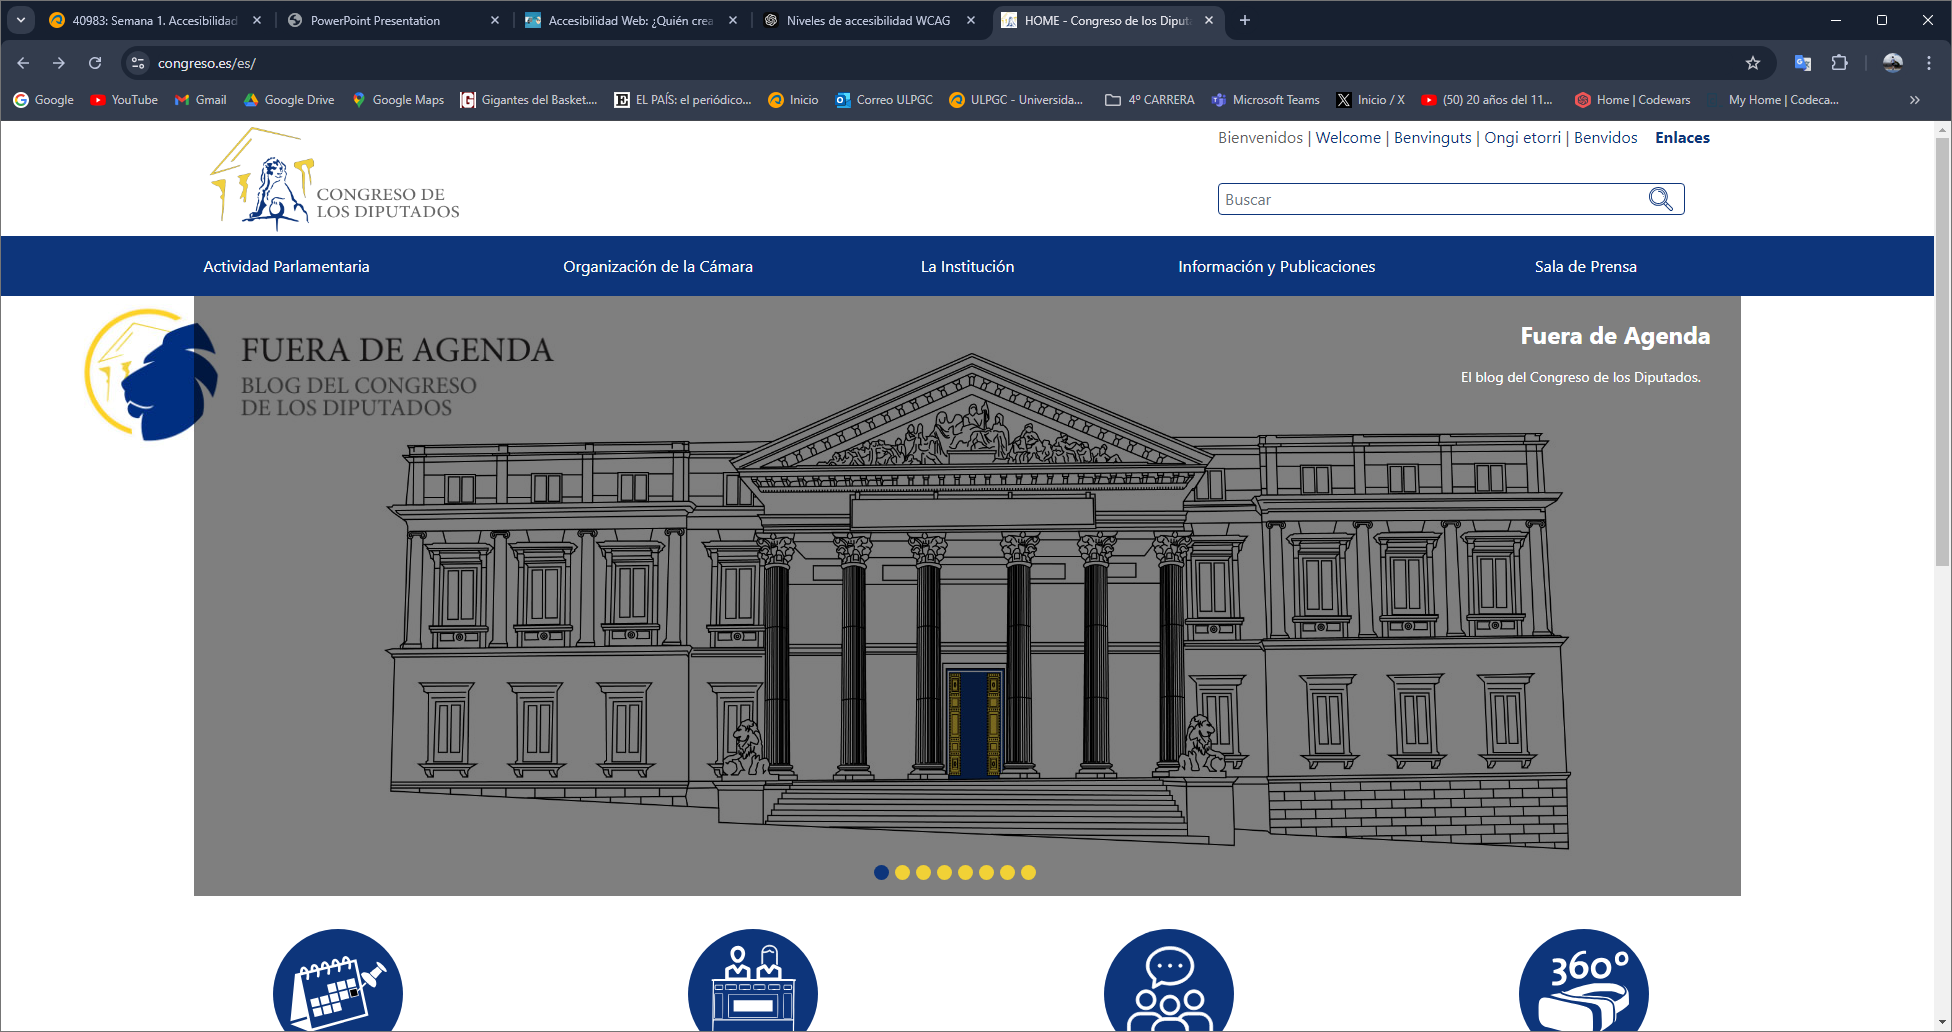
\includegraphics[width=\textwidth]{Capturas/2.png}
	\caption{Página inicial de \href{https://www.congreso.es/es/home}{congreso.es}}
	\label{fig:etiqueta}
\end{figure}

Como punto inicial a tener en cuenta, al tratarse de un sitio web de propósito público, perteneciente a los servicios estatales, se espera un nivel de accesibilidad AA, que proporciona un equilibrio entre mejoras significativas en la accesibilidad y la practicidad de implementación, o AAA, que aborde la mayor cantidad de barreras posibles para llegar al mayor grueso social posible.

\subsection{Problemas detectados tras la evaluación inicial}

La primera problemática que un usuario percibe al acceder a la página principal del \textit{Congreso de los Diputados} es la falta de uso del estándar ISO 639-1 para representar los idiomas mediante sus códigos correctos, como \textit{ES} para español o \textit{EN} para inglés. En la página web se ofrecen cinco opciones idiomáticas: las cuatro lenguas cooficiales del Estado español reconocidas en la Constitución de 1978 (castellano, euskera, catalán y gallego), junto con el inglés como idioma internacional. Los códigos que deberían utilizarse son \textit{ES} (español), \textit{EU} (euskera), \textit{CA} (catalán), \textit{GL} (gallego) y \textit{EN} (inglés). Sin embargo, en su lugar se emplea la interjección \textit{Bienvenido} en cada uno de estos idiomas.

\begin{figure}[h]
	\centering
	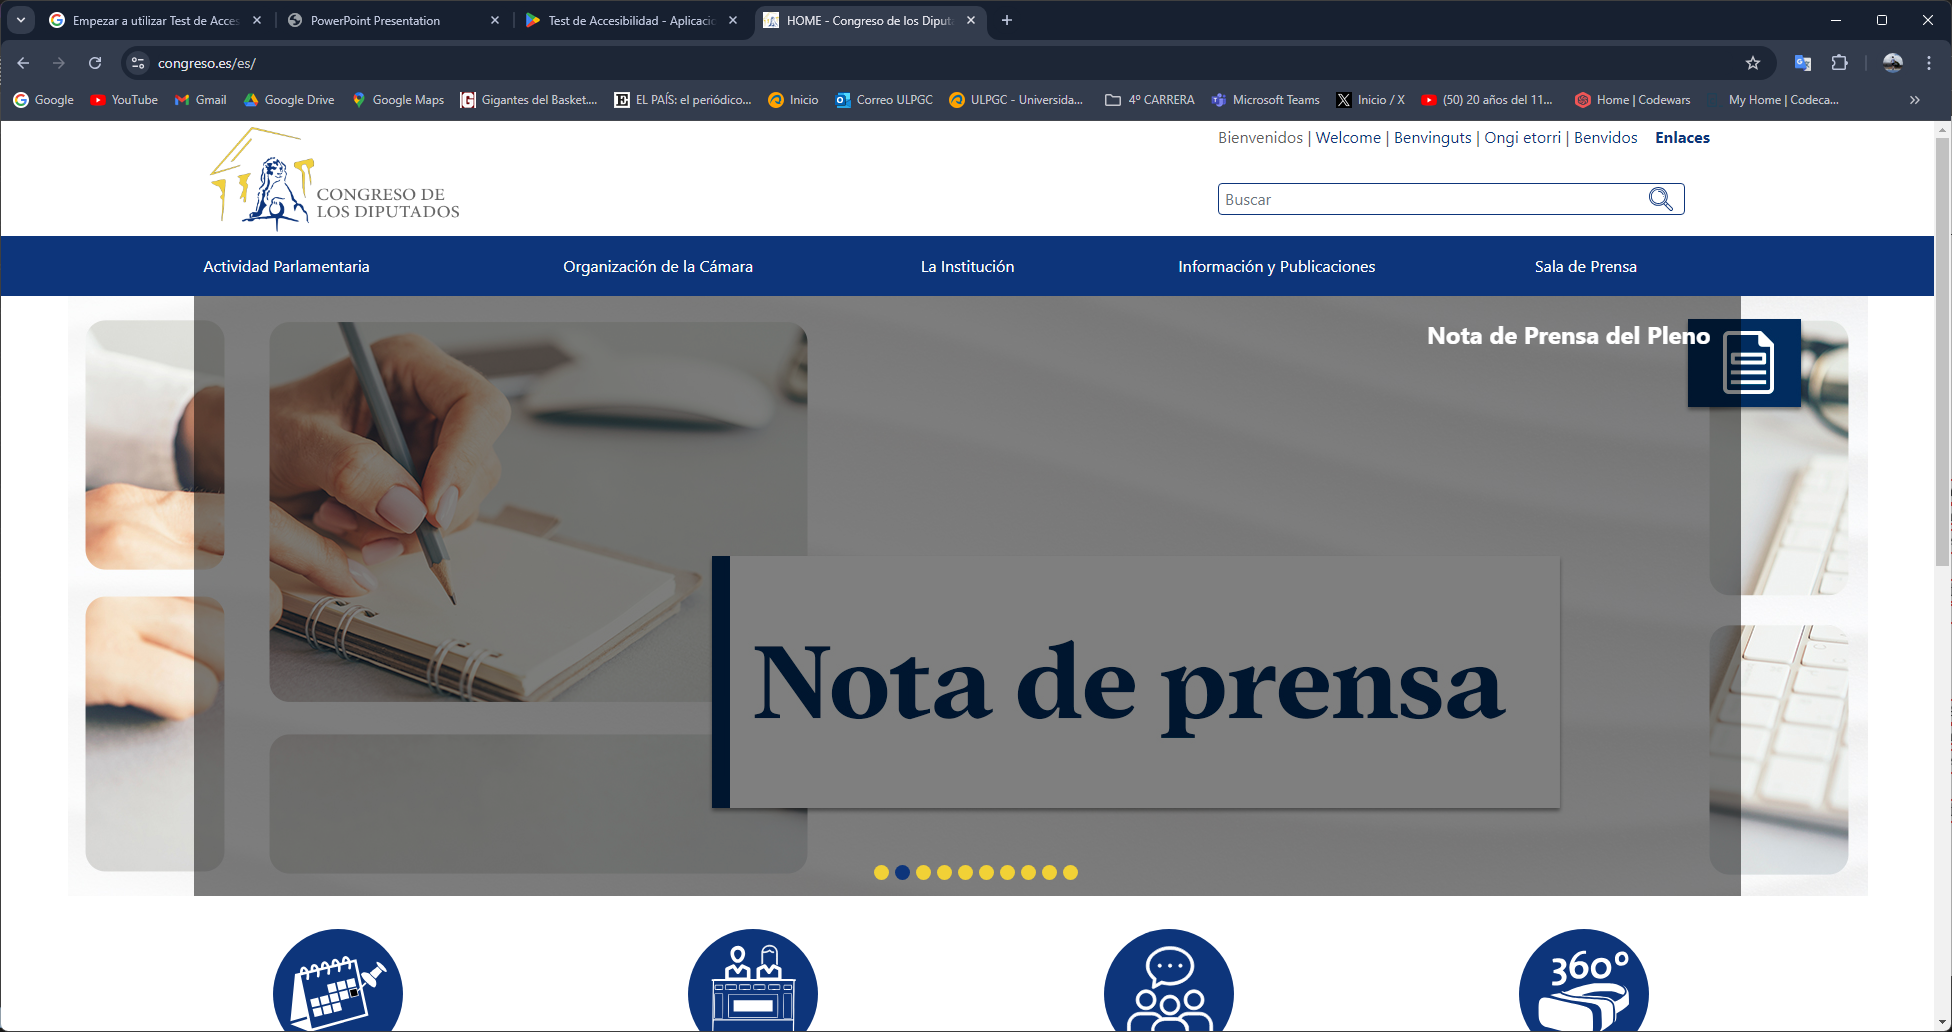
\includegraphics[width=\textwidth]{Capturas/6.png}
	\caption{Página inicial de \href{https://www.congreso.es/es/home}{congreso.es}. En la parte superior, se pueden observar las lenguas disponibles}
	\label{fig:etiqueta}
\end{figure}

Esta práctica viola los principios de accesibilidad WCAG, ya que el uso incorrecto de los códigos de idioma afecta a personas que dependen de tecnologías de asistencia, como lectores de pantalla. Estos dispositivos utilizan el atributo \textit{lang} para identificar el idioma de la página o de secciones específicas del contenido. Si los idiomas no están bien especificados, el lector de pantalla puede interpretar el contenido de forma incorrecta, perjudicando a usuarios con discapacidades visuales.

Además, uno de los criterios clave de accesibilidad es que el contenido sea fácil de entender. Si los idiomas no se presentan de manera estandarizada y clara, los usuarios podrían tener dificultades para identificar el idioma deseado, lo que afecta particularmente a personas con discapacidades cognitivas o de aprendizaje, quienes pueden encontrar confuso o inconsistente el uso de palabras en lugar de códigos.

También, el uso inadecuado de códigos de idioma también puede generar problemas de operabilidad y navegación. Si el menú de idiomas no está etiquetado correctamente, los usuarios que navegan solo con el teclado o utilizan tecnologías de asistencia podrían no identificar el idioma de destino correctamente, complicando la interacción con el sitio web.

Por otra parte, se observa un carrusel o sección destacada, donde se muestran las noticias e información más relevante del sitio web en ese momento. Desde el punto de vista de la accesibilidad, esta sección presenta algunos aspectos a considerar para garantizar que se pueda interactuar con el contenido universalmente y de manera efectiva.

El uso del sombreado oscuro sobre la imagen que se presenta en el carrusel puede afectar la legibilidad del texto y de la información que se expone. Si el contraste entre el texto y el fondo no es el suficiente, los usuarios con problemas visuales o de contraste podrían tener dificultades para leerlo. Una posible solución sería aumentar el contraste entre el texto y el fondo de la imagen o proporcionar herramientas que permitan a los usuarios ajustar el nivel de contraste según sus necesidades.

Es fundamental, en todo caso, que la imagen cuente con un atributo \texttt{alt} descriptivo que explique su contenido para los usuarios que utilizan lectores de pantalla. En este caso, un atributo alternativo adecuado podría ser ``Nota de prensa'' destacada en la página principal del \textit{Congreso de los Diputados}. Esto permite que los usuarios que no pueden ver la imagen puedan entender el propósito del contenido visual presentado en la página.

\subsection{Problemas detectados tras el empleo de herramientas de accesibilidad}

\subsubsection{Evaluación con Google Lighthouse}

Para el análisis del resto de aspectos de accesibilidad de esta página, se han escogido algunas herramientas, entre ellas \textit{Google Lighthouse}, que incluida como herramienta de desarrollo en \textit{Chrome DevTools} al pulsar la pestaña \textit{Inspeccionar}. Estas comprobaciones permiten identificar oportunidades para mejorar la accesibilidad de una aplicación web. La detección automática solo puede detectar un subconjunto de problemas y no garantiza la accesibilidad de la aplicación web.

\begin{figure}[h]
	\centering
	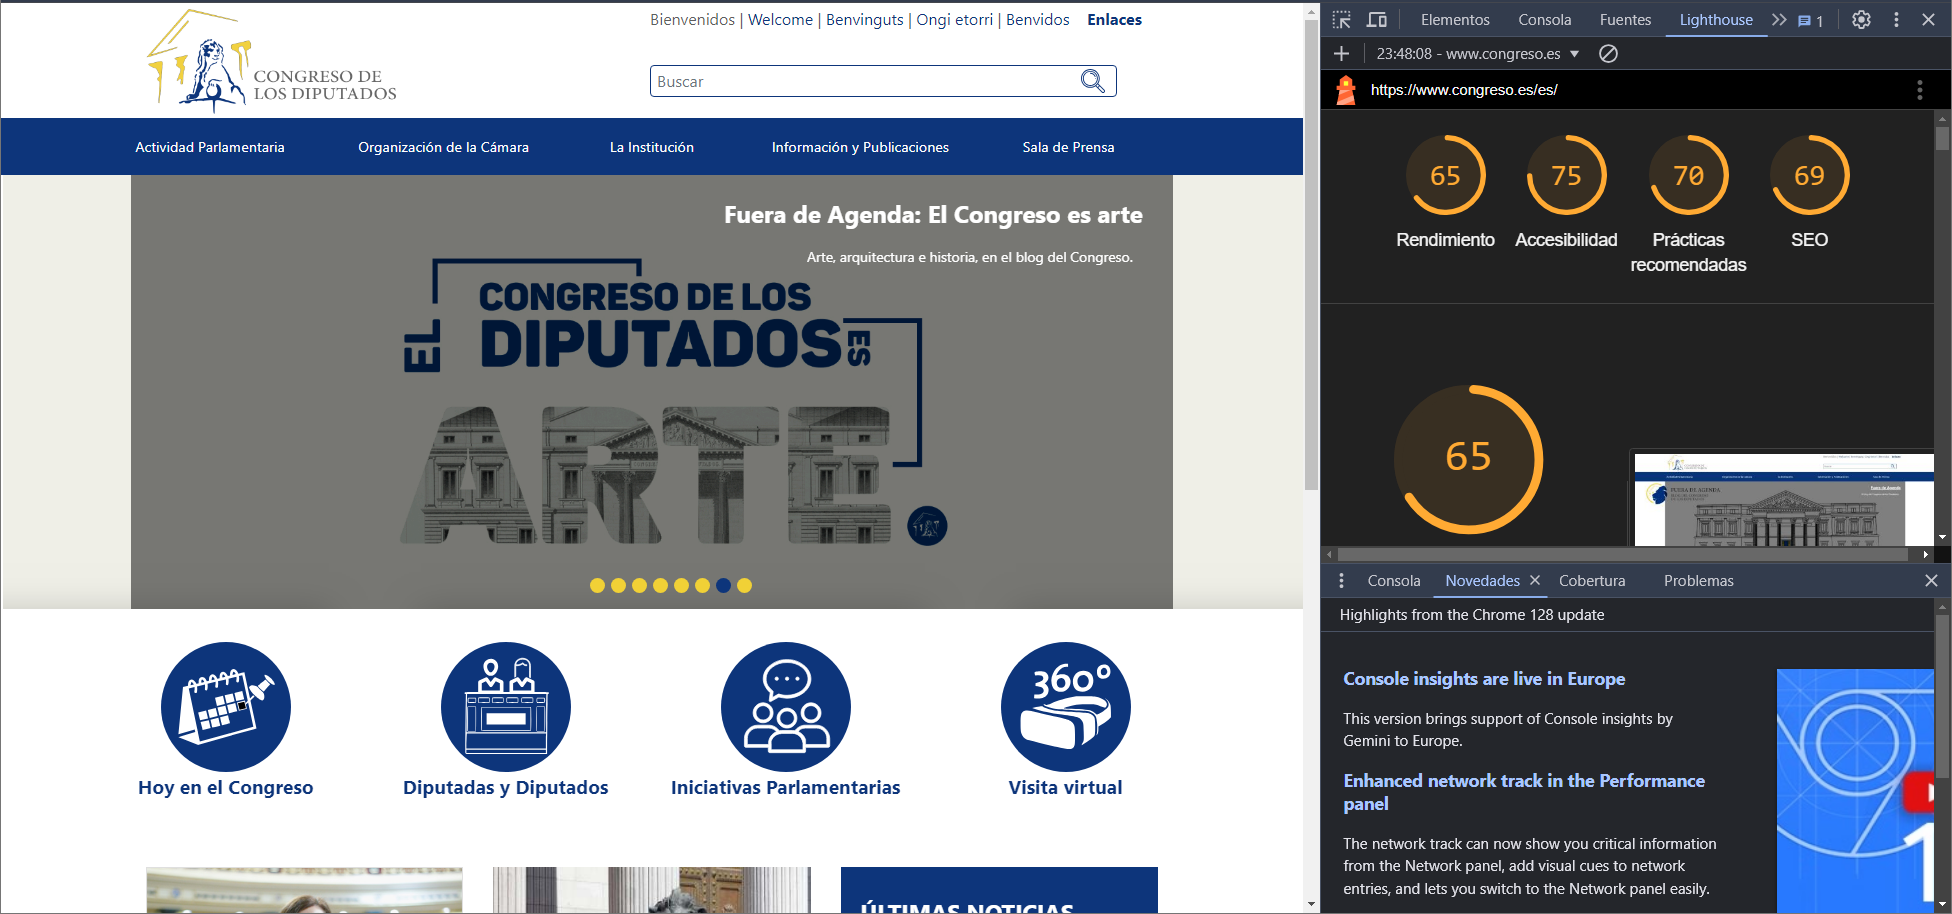
\includegraphics[width=\textwidth]{Capturas/1.png}
	\caption{Análisis de la página inicial de \href{https://www.congreso.es/es/home}{congreso.es} por \textit{Google Lighthouse}}
	\label{fig:etiqueta}
\end{figure}

En el análisis llevado a cabo, Google Lighthouse otorga a la página principal del \textit{Congreso de los Diputados} (\href{https://www.congreso.es/es/home}{congreso.es}) una puntuación de 75 sobre 100. En él, se han identificado varios problemas relacionados con el uso de ARIA, la correcta asignación de nombres y etiquetas, la estructura de tablas y listas, la internacionalización, y la navegación del sitio:

\subsection*{ARIA}
\textit{Accessible Rich Internet Applications} (ARIA) es una colección de atributos que definen como realizar contenido y aplicaciónes web, especialmente las desarrolladas con JavaScript, más accesibles para las personas con discapacidades. Complementa HTML para que las interacciones y los widgets que se usan comúnmente en las aplicaciones puedan ser correctamente interpretadas por las tecnologías de asistencia cuando no existe otro mecanismo. Por ejemplo, ARIA habilita accesibilidad a widgets de JavaScript, sugerencias de formularios, mensajes de error, actualizaciones de contenido en vivo y más.
\begin{itemize}
	\item Se ha detectado que algunos atributos \texttt{[aria-*]} no se corresponden con sus funciones previstas dentro de la estructura de la página. Esto puede generar confusión para las tecnologías de asistencia como los lectores de pantalla, que no podrán interpretar correctamente el contenido.
	
	\item Falta de elementos secundarios en roles ARIA (por ejemplo, menús, botones, etc.) que requieren la presencia de estos para ser accesibles. Estos elementos secundarios no están presentes en algunos casos, lo que afecta negativamente la navegación de los usuarios con discapacidades.
	
	\item Uso de roles ARIA en elementos incompatibles. Algunos roles ARIA han sido aplicados en elementos HTML que no son compatibles con esos roles, lo que genera problemas de accesibilidad.
\end{itemize}

\subsection*{Nombres y etiquetas}
La correcta asignación de nombres y etiquetas a los enlaces es crucial para garantizar que los usuarios puedan navegar por el sitio de manera efectiva. Los problemas detectados incluyen:
\begin{itemize}
	\item Algunos enlaces dentro de la aplicación carecen de nombres descriptivos, reconocibles o etiquetas claras, lo que dificulta su identificación para los usuarios de tecnologías de asistencia como los lectores de pantalla. Los usuarios necesitan saber de forma precisa a dónde los llevará cada enlace. 
	\item Algunas imágenes contienen atributos alt con descripciones que son redundantes o innecesarias. Esto provoca una carga de información extra para los usuarios de lectores de pantalla, lo que puede dificultar la navegación y comprensión del contenido.
\end{itemize}

\subsection*{Tablas y listas}
Las tablas y listas deben estar bien estructuradas para que sean accesibles para los lectores de pantalla y otras tecnologías de asistencia. En este caso, \textit{Google Lighthouse} ha detectado un problema común:
\begin{itemize}
	\item Los elementos de lista (\texttt{<li>}) no están dentro de elementos superiores válidos (\texttt{<ul>}, \texttt{<ol>}, \texttt{<menu>}). Los elementos de lista (\texttt{<li>}) deben estar correctamente anidados dentro de un contenedor de lista válido, como <ul> para listas no ordenadas o <ol> para listas ordenadas. Sin esta estructura, los lectores de pantalla no podrán interpretar las listas adecuadamente, dificultando la navegación y comprensión.
\end{itemize}

\subsection*{Internalización y localización}
\begin{itemize}
	\item El atributo lang, que especifica el idioma del contenido de una página o de una sección de la misma, no contiene valores válidos en algunas partes de la aplicación. Esto afecta negativamente a los usuarios con configuraciones regionales específicas o que utilizan lectores de pantalla para ajustar la pronunciación del contenido según el idioma.
\end{itemize}

\subsection*{Navegación}
\begin{itemize}
	\item La estructura de encabezados (etiquetas \texttt{<h1>}, \texttt{<h2>}, ...) no sigue un orden secuencial adecuado, lo que complica la navegación para los usuarios que dependen del teclado o de tecnologías de asistencia para desplazarse por el contenido.
\end{itemize}

\subsubsection{Evaluación con axe DevTools}

Para complementar el análisis de accesibilidad de la página principal del \textit{Congreso de los Diputados}, se ha utilizado la herramienta \textit{axe DevTools}, una extensión del navegador que permite identificar problemas de accesibilidad en tiempo real. Esta herramienta es especialmente útil para detectar problemas en el uso de atributos ARIA, la semántica del contenido, y otros aspectos que pueden afectar la experiencia de los usuarios con discapacidades. Aunque axe \textit{axe DevTools} puede detectar una amplia gama de problemas, es importante recordar que no garantiza una accesibilidad completa y que siempre es necesario realizar pruebas adicionales.

\begin{figure}[h]
	\centering
	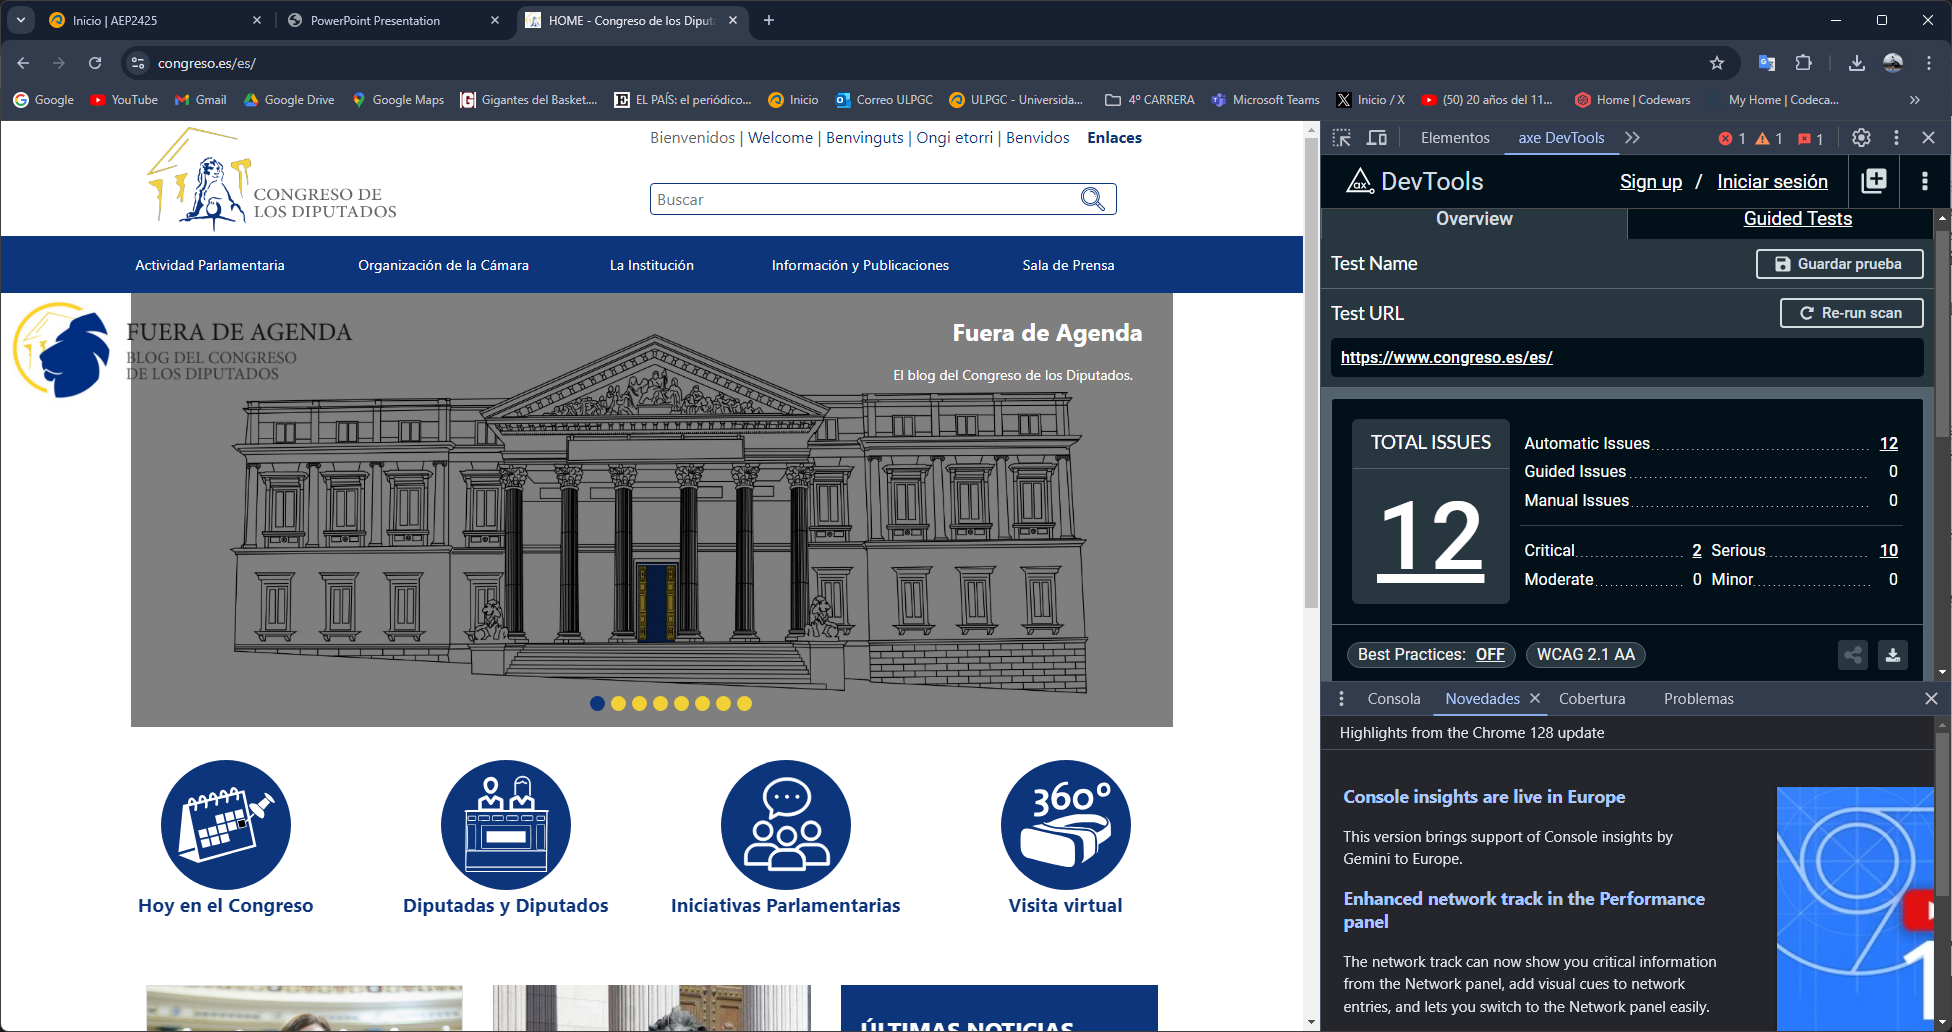
\includegraphics[width=\textwidth]{Capturas/3.png}
	\caption{Análisis de la página inicial de \href{https://www.congreso.es/es/home}{congreso.es} por \textit{axe DevTools}}
	\label{fig:etiqueta}
\end{figure}

En el análisis, se han identificado 12 problemas principales que afectan la accesibilidad de la página.

En el análisis de la página de Agenda Parlamentaria, por contraparte, se han identificado 41 problemas principales que afectan la accesibilidad de la página.

\begin{figure}[h]
	\centering
	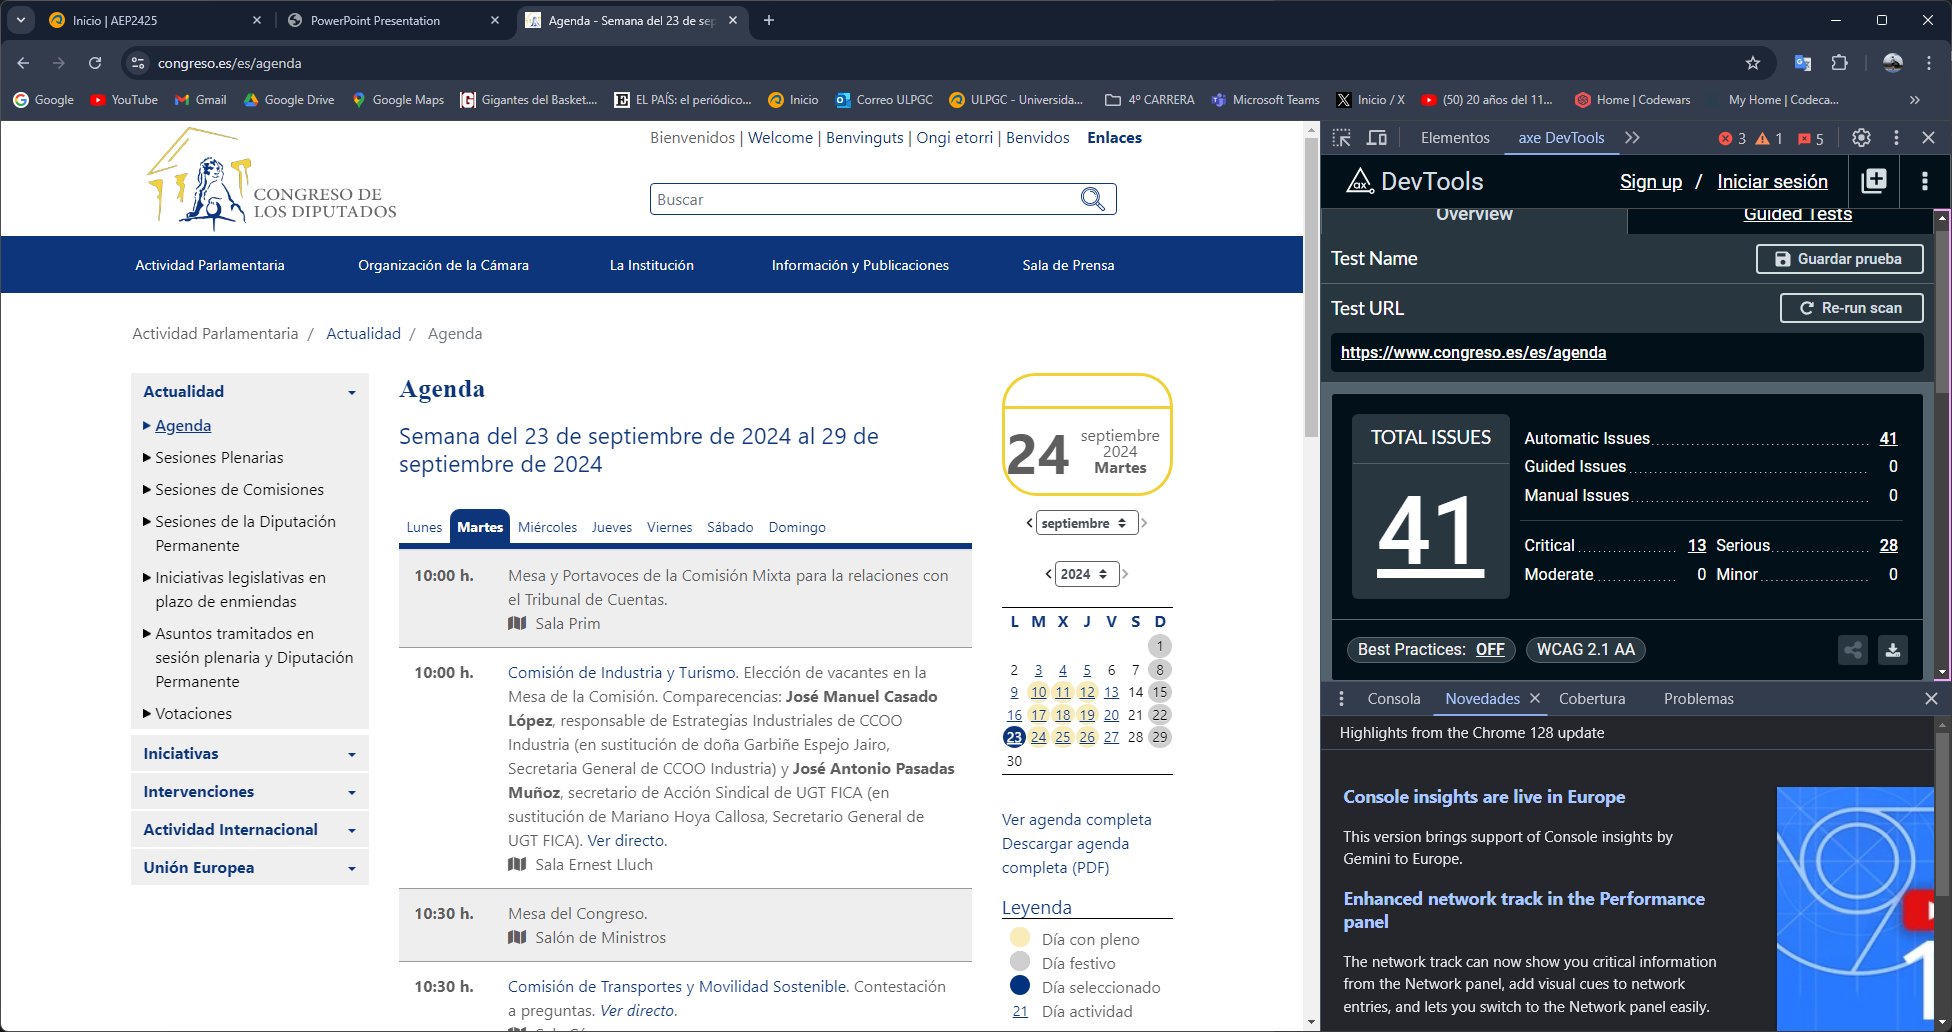
\includegraphics[width=\textwidth]{Capturas/4.png}
	\caption{Análisis de la página de Agenda Parlamentaria de \href{https://www.congreso.es/es/home}{congreso.es} por \textit{axe DevTools}}
	\label{fig:etiqueta}
\end{figure}

A continuación, se detallan los problemas más destacados y sus implicaciones:

\subsection*{Atributos ARIA}
\begin{itemize} 
	\item Se ha detectado que algunos elementos están utilizando atributos ARIA que no son permitidos. Esto puede generar comportamientos inesperados en las tecnologías de asistencia, impidiendo que el contenido se interprete correctamente.	
	\item Elementos con roles ARIA incompletos. Algunos roles ARIA, que requieren que los elementos secundarios contengan roles específicos, no cumplen con esta estructura. Esto puede afectar negativamente la capacidad de los usuarios para interactuar correctamente con estos elementos, dificultando la navegación y el uso de componentes interactivos.
\end{itemize}

\subsection*{Enlaces y etiquetas}
\begin{itemize} 
	\item Algunos enlaces carecen de texto accesible y discernible, lo que dificulta que los lectores de pantalla los identifiquen correctamente. Esto crea un obstáculo para los usuarios, quienes necesitan información clara sobre el propósito de cada enlace para interactuar con él. 
\end{itemize}

\subsection*{Tablas y listas}
\begin{itemize} 
	\item Algunos elementos de lista (\texttt{<li>}) no están anidados correctamente dentro de los contenedores de listas válidos (\texttt{<ul>}, \texttt{<ol>}). Este problema afecta la capacidad de los lectores de pantalla para interpretar correctamente la estructura de la lista, lo que puede causar confusión a los usuarios al navegar por el contenido. 
\end{itemize}

\subsection*{Internacionalización y localización}
\textit{axe DevTools} también ha detectado problemas relacionados con la internacionalización y localización del contenido. En este caso:
\begin{itemize} 
	\item El atributo \texttt{lang}, que se utiliza para especificar el idioma del contenido de una página o sección, tiene valores no válidos en algunas partes de la aplicación. Esto afecta a los usuarios que dependen de lectores de pantalla para adaptar la pronunciación y lectura del contenido según su idioma. 
\end{itemize}

\subsection{Soluciones Propuestas}
\begin{itemize}
	\item Corregir los atributos \texttt{[aria-*]} y \texttt{alt} y asegurarse de que están bien aplicados para una correcta interpretación de las tecnologías de asistencia.
	\item Aumentar el contraste entre el texto y el fondo de las imágenes.
	\item Seguir el estándar ISO 639-1 para representar los idiomas mediante sus códigos correctos. 
	\item Asignar nombres claros y descriptivos a enlaces e imágenes.
	\item Garantizar que los elementos de lista estén correctamente anidados dentro de \textit{ul}, \textit{ol} o \textit{menu}.
	\item Utilizar correctamente el atributo \textit{lang} para asegurar que los lectores de pantalla reconozcan el idioma.
	\item Reorganizar los encabezados de forma secuencial y lógica para mejorar la navegación.
\end{itemize}

\subsection{Nivel de accesibilidad sugerido}
Tras los análisis realizados con Google Lighthouse y axe DevTools, es posible evaluar el nivel de accesibilidad de la página principal del \textit{Congreso de los Diputados} en base a las WCAG:
\begin{itemize}
	\item Nivel A aborda los requisitos mínimos de accesibilidad y es esencial para que los usuarios puedan interactuar con el contenido.
	\item Nivel AA aborda un conjunto más amplio de barreras de accesibilidad y se considera el estándar recomendado para la mayoría de los sitios públicos.
	\item Nivel AAA es el nivel más exigente y garantiza la máxima accesibilidad, pero puede ser más difícil de implementar.
\end{itemize}

A partir de los resultados obtenidos con las herramientas de auditoría, en las que:
\begin{itemize}
	\item \textit{Google Lighthouse} otorgó una puntuación de 75 sobre 100, identificando problemas significativos en el uso de ARIA, en la asignación de nombres y etiquetas, la estructura de tablas y listas, la internacionalización, y la navegación.
	\item \textit{axe DevTools} detectó 12 problemas críticos, entre los que destacan el uso incorrecto de atributos ARIA, enlaces sin texto accesible, la falta de estructura en las listas, y la asignación inadecuada del atributo \textit{lang} para la especificación del idioma.
\end{itemize}

En definitiva, se sugiere que el sitio web no alcance el nivel de conformidad AAA, ya que presenta varios problemas que impiden el cumplimiento de los criterios más exigentes de accesibilidad, especialmente en lo que respecta a la correcta interpretación de elementos interactivos, la navegación con tecnologías de asistencia, y la estructura semántica de la página, a pesar de tratarse de un sitio web de propósito público. 

Sin embargo, la mayoría de los problemas identificados podrían solucionarse con mejoras relativamente simples, lo que permitiría al sitio alcanzar un nivel de conformidad AA. Actualmente, el sitio se sitúa entre los niveles A y AA, cumpliendo con varios de los requisitos básicos de accesibilidad, pero aún presenta barreras que impiden alcanzar un nivel óptimo. 

Por tanto, se recomienda implementar las correcciones necesarias para cumplir con el nivel AA de las WCAG, lo que garantizaría una mayor inclusividad y accesibilidad para todos los usuarios, en línea con las normativas internacionales de accesibilidad digital.
\newpage

\section{Análisis de accesibilidad de la aplicación móvil \textit{Sofascore}}

A continuación, se realizará nuevamente un análisis detallado de accesibilidad, esta vez referente a la aplicación móvil de resultados deportivos \textit{Sofascore}, disponible para Android e iOS. En este caso no se trata de una aplicación móvil de propósito público, por lo que no se sabe, a priori, que nivel de accesibilidad WCAG se espera que cumpla.

\begin{figure}[H]
	\centering
	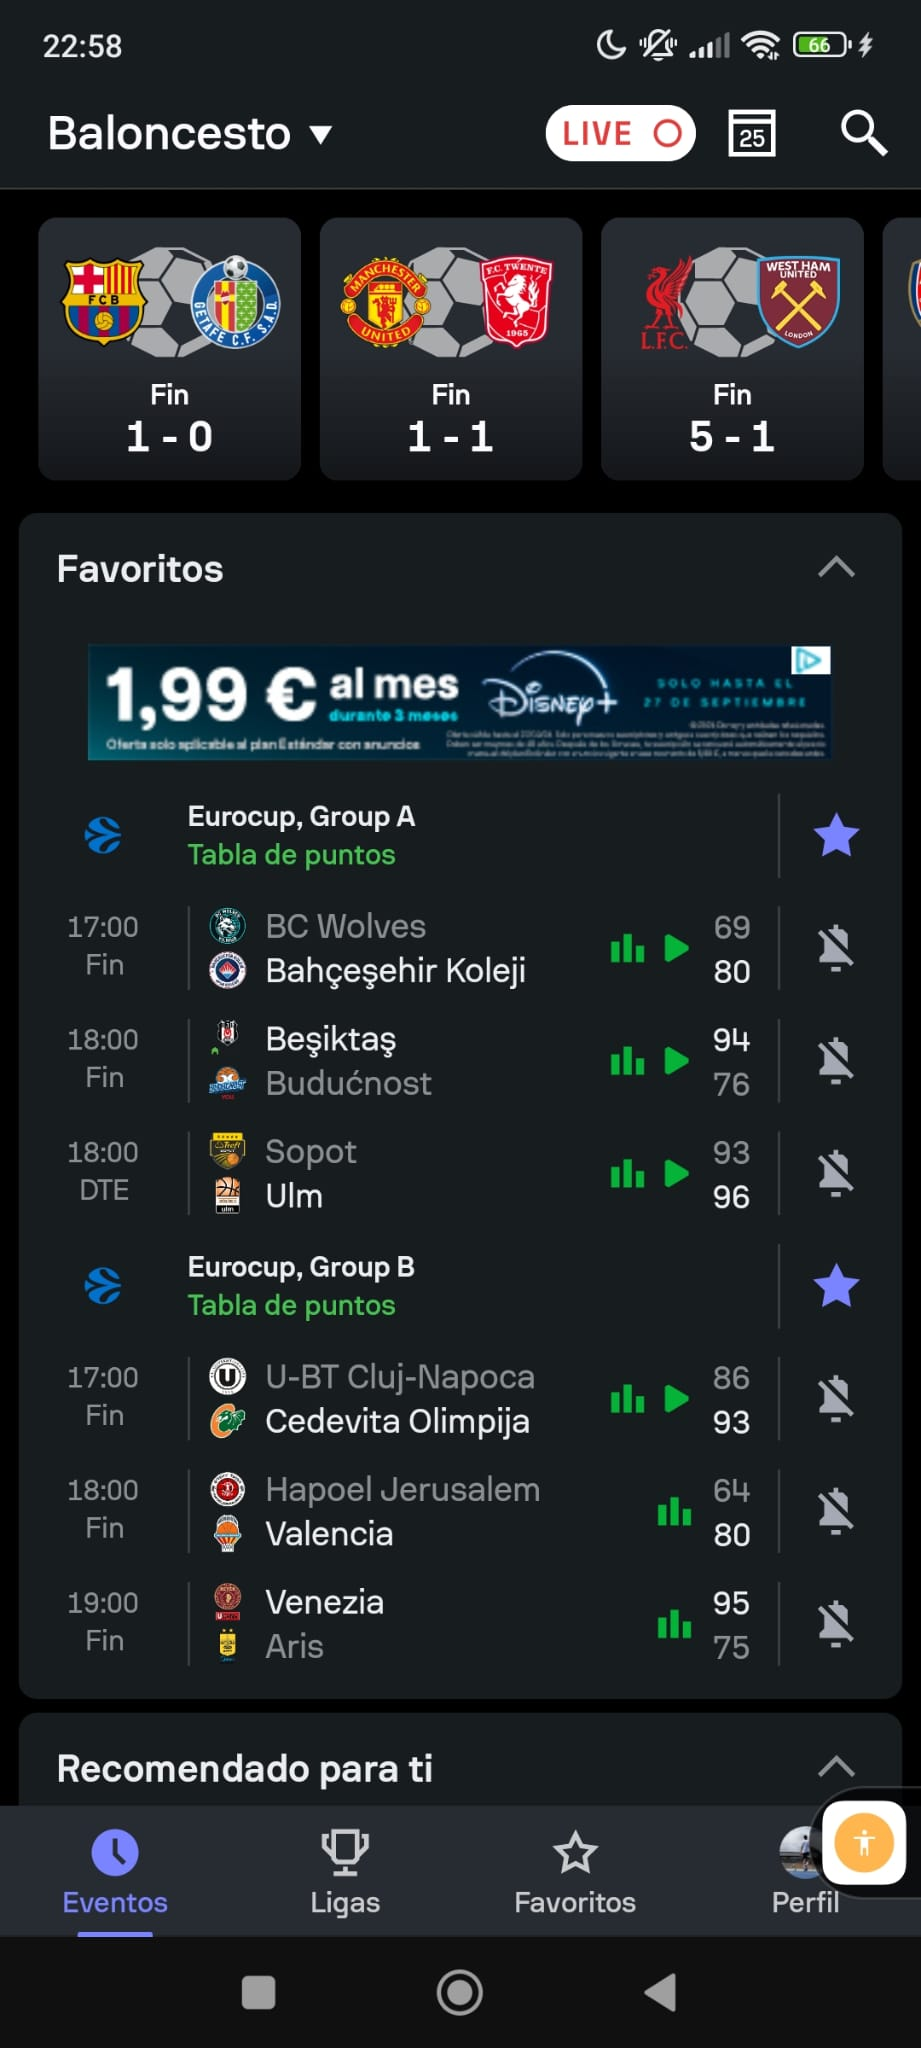
\includegraphics[width=0.4\textwidth]{Capturas/7.png}
	\caption{Página inicial de \textit{Sofascore}}
	\label{fig:etiqueta}
\end{figure}

\subsection{Problemas detectados tras la evaluación inicial}

El primer elemento visual destacable es la tonalidad oscura de la página principal de la aplicación móvil. Esta característica puede ajustarse en la configuración del programa según las preferencias del usuario. El modo oscuro puede reducir la fatiga visual durante el uso prolongado del dispositivo, mientras que el modo claro puede mejorar la legibilidad gracias al alto contraste de colores. Es importante asegurarse de que este contraste cumpla con los estándares de accesibilidad, especialmente para usuarios con baja visión. Sin embargo, en algunas áreas más pequeñas, como los íconos de sonido y gráficos estadísticos, este contraste podría no ser suficiente, sobre todo cuando el fondo y los elementos no contrastan de manera clara.

Por otra parte, cabe destacar los textos pequeños de algunas áreas, como los resultados de los partidos o los nombres de los equipos. Puede ser difícil de leer para personas con alguna discapacidad visual. Es esencial que la aplicación permita escalar el texto, sin comprometer la disposición ni el diseño. De manera similar, los íconos que representan funciones como el acceso a la tabla de puntos o a otras secciones de la aplicación también deberían ser lo suficientemente grandes y claros para ser fácilmente accesibles, especialmente mediante teclado u otros dispositivos de asistencia.

Además, los íconos y gráficos parecen carecer de descripciones accesibles para usuarios que dependen de lectores de pantalla. Estas descripciones son cruciales para que dichos usuarios puedan comprender el contenido y beneficiarse de la funcionalidad completa de la aplicación.

Por último, el uso del color verde y rojo para indicar las estadísticas de los equipos podría ser un gran desafío para usuarios con daltonismo. Sería recomendable añadir texto o símbolos adicionales para clarificar la información que se comunica a través del color.

\subsection{Problemas detectados tras el empleo de herramientas de accesibilidad}

\subsubsection{Evaluación con Test de Accesibilidad}

Para evaluar la accesibilidad de la aplicación SofaScore desde la perspectiva de una persona con discapacidades visuales, se hizo uso de la funcionalidad \textit{TalkBack} de la aplicación \textit{\href{https://play.google.com/store/apps/details?id=com.google.android.apps.accessibility.auditor&pcampaignid=web_share}{Test de Accesibilidad}} de Google. Esta herramienta permite simular el uso de la aplicación mediante un lector de pantalla, proporcionando una experiencia similar a la que tendría una persona con baja visión o ceguera. 

Al realizar la prueba, la experiencia resulta muy molesta para el usuario. Algunos de los principales problemas incluyen la falta de descripciones accesibles para los íconos, gráficos, nombres de jugadores y equipos, lo que complica la navegación y la comprensión de la información.

\begin{figure}[H] % Usa H para forzar la posición
	\centering
	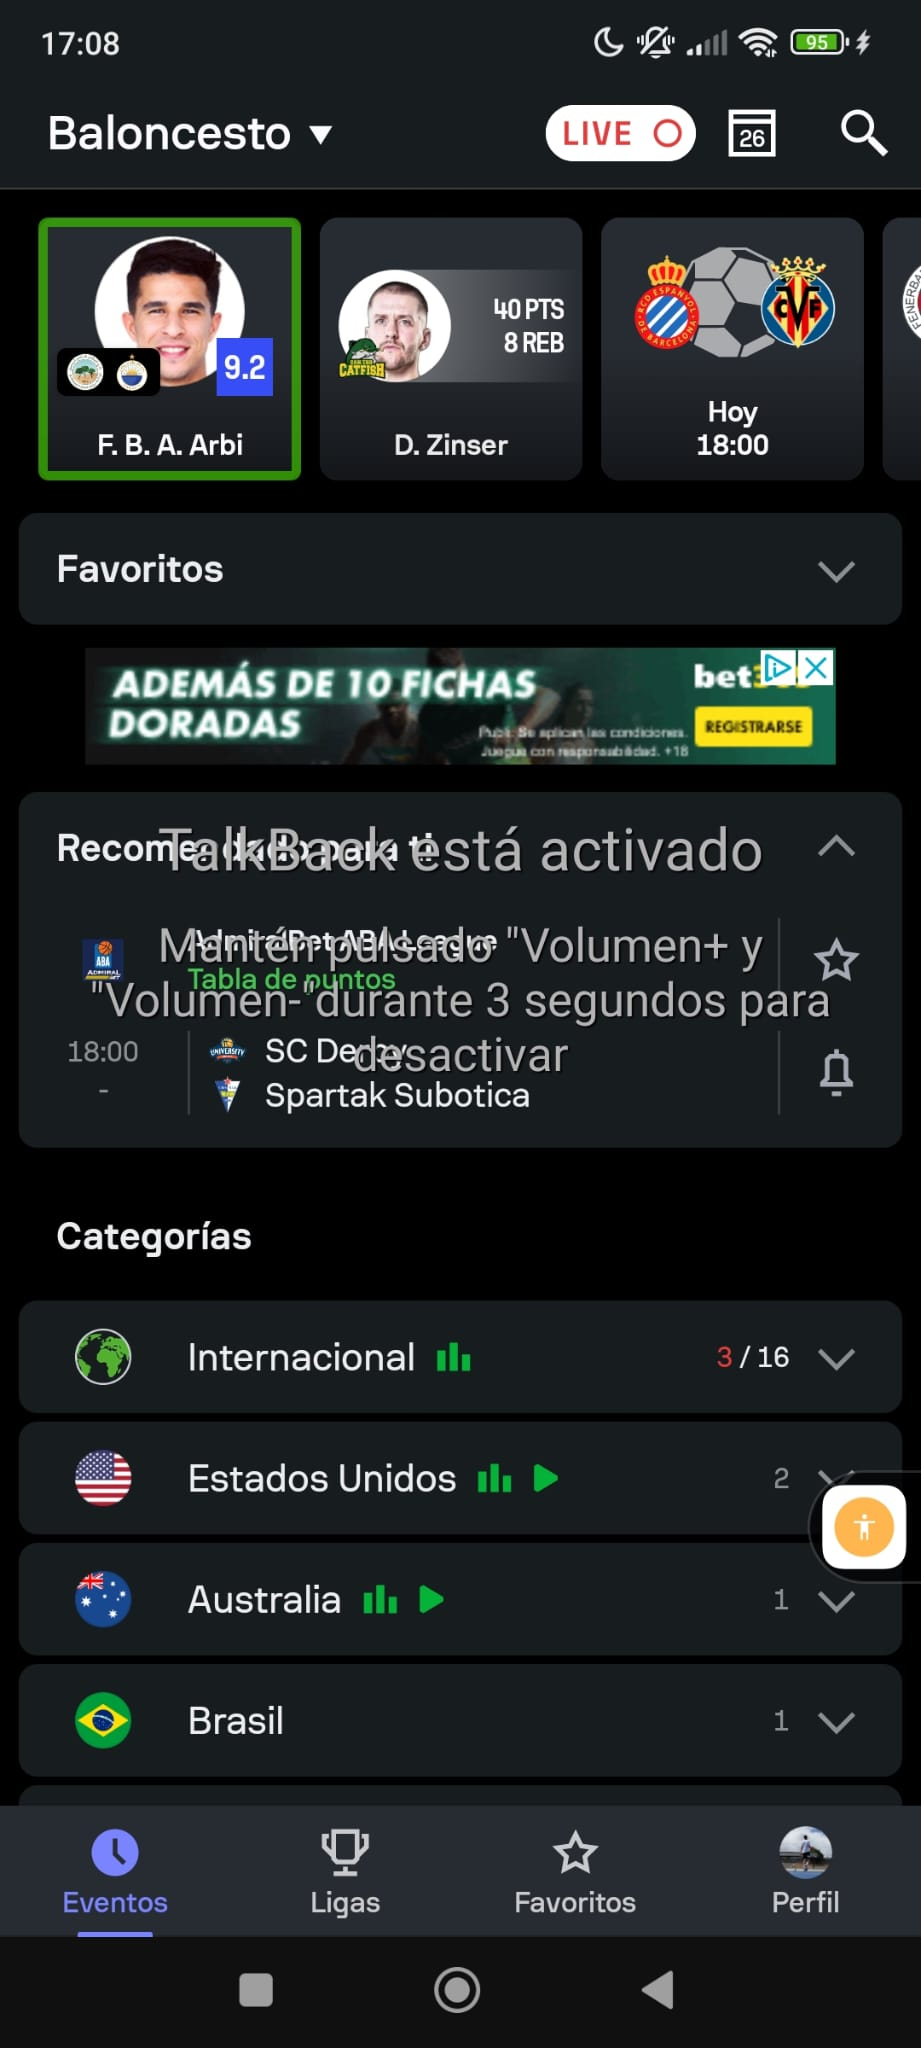
\includegraphics[width=0.4\textwidth]{Capturas/8.png}
	\caption{Página inicial de \textit{SofaScore}, desde la perspectiva de accesibilidad de \textit{TalkBack}}
	\label{fig:etiqueta}
\end{figure}


Además, la estructura de los menús no está optimizada para un lector de pantalla, lo que ralentiza considerablemente la interacción. \textit{TalkBack} no logra identificar elementos clave de la interfaz, lo que obliga al usuario a realizar múltiples intentos para acceder a determinadas funciones o datos. 

En definitiva, la accesibilidad para personas con problemas visuales podría mejorarse significativamente, especialmente en lo que respecta a la compatibilidad con herramientas de asistencia como \textit{TalkBack}.

\subsection{Soluciones Propuestas}
\begin{itemize}
	\item Mejorar el contraste de colores en textos, íconos y fondo, siguiendo los estándares de accesibilidad de WCAG para usuarios con baja visión. Garantizar, así, que los gráficos estadísticos y los íconos tengan un contraste adecuado.
	\item Aumentar el tamaño de los textos y los íconos.
	\item Incluir descripciones para lectores de pantalla en las imágenes.
	\item Mejor organización y simplificación de la estructura del menú para lectores de pantalla.
	\item Incorporar texto adicional, símbolos o patrones para acompañar los colores que se utilizan para representar estadísticas, de modo que los usuarios con daltonismo puedan interpretar la información sin depender del color.
	\item Mejoras para asegurar que todas las funciones sean fácilmente accesibles mediante dispositivos de asistencia, como teclados o controles de voz, facilitando la experiencia a personas con movilidad reducida o discapacidades visuales.
\end{itemize}

\subsection{Nivel de accesibilidad sugerido}

Tras analizar la experiencia de usuario de la aplicación \textit{Sofascore}, atendiendo a las Pautas de Accesibilidad para el Contenido Web (WCAG) 2.1, se recomienda que se sitúe en el nivel AA. Este es el estándar recomendado porque ofrece un equilibrio adecuado entre accesibilidad y diseño, asegurando que la mayoría de las personas, incluidas aquellas con discapacidades visuales, auditivas o motoras, puedan utilizar la aplicación de manera efectiva sin que ello interfiera excesivamente en el aspecto visual o funcional del producto.

Este nivel incluye requisitos como un buen contraste de color, compatibilidad con tecnologías de asistencia (lectores de pantalla), escalabilidad de texto, y retroalimentación clara en casos de error. La aplicación garantizaría una accesibilidad amplia sin comprometer su atractivo ni usabilidad para otros usuarios. No obstante, se deberían solucionar los fallos nombrados anteriormente como paso previo.

\newpage

\section{Conclusiones}

Las evaluaciones de accesibilidad realizadas sobre el sitio web del \textit{Congreso de los Diputados} (\href{https://www.congreso.es/es/home}{congreso.es}) y de la aplicación móvil de estadísticas deportivas \textit{\href{https://play.google.com/store/apps/details?id=com.sofascore.results&pcampaignid=web_share}{Sofascore}} revelan sendos puntos de mejora en cuanto a su adaptabilidad a todas las personas, incluidas aquellas con algún grado de discapacidad.

Resulta necesaria la democratización en el uso de las nuevas tecnologías, que se encuentran a la orden del día, para que el uso de estas sea generalizado, empezando, no solo por los dispositivos que se emplean, sino por las webs y las herramientas que se usan en ellos.

Es fundamental que las plataformas digitales, tanto públicas como privadas, cumplan con los estándares de accesibilidad establecidos en las Pautas de Accesibilidad para el Contenido Web (WCAG). Estos estándares no solo garantizan la equidad en el acceso a la información, sino que también promueven la inclusión digital de todos los ciudadanos, independientemente de sus capacidades físicas, sensoriales o cognitivas.

En el caso particular del sitio web del \textit{Congreso de los Diputados}, la accesibilidad resulta de especial importancia, ya que se trata de un espacio digital de acceso público que debe estar disponible para todos los ciudadanos, incluidas aquellas personas con discapacidades. A pesar de su relevancia, el análisis revela ciertas carencias, como la falta de descripciones adecuadas en imágenes y elementos multimedia, problemas de navegación con dispositivos de asistencia, y dificultades para usuarios con discapacidades visuales o motoras.

\newpage

\section{Bibliografía}

\begin{thebibliography}{9}
	\bibitem{enlace1}
	DodepechoAdmin, 
	\emph{La importancia de la accesibilidad web - Dodepecho}, 
	\url{https://dodepecho.com/la-importancia-de-la-accesibilidad-web/#:~:text=%C2%BFPor%20qu%C3%A9%20la%20accesibilidad%20web,de%20sus%20capacidades%20o%20limitaciones.}, 
	2023, 3 mayo.
	
	\bibitem{enlace2}
	De la República Epn, 
	\emph{TíConoce los distintos tipos de discapacidad. gob.mx.}, 
	\url{https://www.gob.mx/epn/es/articulos/conoce-los-distintos-tipos-de-discapacidad}, 
	s. f.
	
	\bibitem{enlace3}
	World Health Organization: WHO, 
	\emph{Discapacidad}, 
	\url{https://www.who.int/es/news-room/fact-sheets/detail/disability-and-health}, 
	2023, 7 marzo.
	
	\bibitem{enlace4}
	Mora, S. L., 
	\emph{Accesibilidad Web}, 
	\url{https://accesibilidadweb.dlsi.ua.es/?menu=que-es-wcag}, 
	s. f.
	
	\bibitem{enlace5}
	Wikipedia, 
	\emph{ISO 639-1}, 
	\url{https://es.wikipedia.org/wiki/ISO_639-1}, 
	2024, 26 enero.
	
	\bibitem{enlace6}
	MDN Web Docs, 
	\emph{ARIA - Accesibilidad}, 
	\url{https://developer.mozilla.org/es/docs/Web/Accessibility/ARIA}, 
	2024, 28 julio.

\end{thebibliography}

\end{document}
